\documentclass[a4paper,20pt]{report}
\usepackage[utf8]{inputenc}
%\usepackage{titlesec}
\usepackage{graphicx}
\usepackage{color}
\usepackage{amssymb}
\usepackage{amsmath}
\usepackage{textcomp}
%\usepackage{enumitem}
%\usepackage{multirow}
%\usepackage{rotating,capt-of}
\usepackage[small]{caption}
\usepackage{booktabs}
\usepackage{fixltx2e} % two-column fig/tab float order
\usepackage{float} % for placing figures where i want
\usepackage{afterpage}
%\usepackage{soul}  % KR: added as it contains \st command
%\usepackage{epsfig, a4wide}
%\usepackage{floatflt}
\usepackage{url}
%\usepackage{hyperref}
\usepackage{colortbl}
\usepackage{graphics,amssymb,amsmath,epsfig,color}
\usepackage{graphicx}
\usepackage{caption}
%\usepackage{lipsum}
\usepackage{pdfpages}
\usepackage{subcaption}
\usepackage{tikz}
%\usepackage{float} % for placing figures where i want
\usepackage{indentfirst}
\usepackage[linktocpage=false]{hyperref}
\usepackage{enumerate}
\usepackage{enumitem}
\usepackage{listings}
%\usepackage{graphicx}
%\usepackage{color}
\hypersetup{
    colorlinks=false,
    pdfborder={0 0 0},}
\setcounter{tocdepth}{3}
\setcounter{secnumdepth}{4}
\setcounter{secnumdepth}{4}

\newcommand*\circled[1]{\tikz[baseline=(char.base)]{
            \node[shape=circle,draw,inner sep=2pt] (char) {#1};}}
\newcommand{\note}{\textcolor{red}}
\newcommand*{\rom}[1]{\uppercase\expandafter{\romannumeral #1\relax}}
%\huge
\title{\huge  \textbf{MIRfix}}
\author{\huge Documentation}
\date{ }
 
\begin{document}
%\normalsize 
\maketitle
 
\tableofcontents
\pagebreak
%\prer
\chapter*{Installation}\stepcounter{chapter}\addcontentsline{toc}{chapter}{Installation}
\section{Conda environment}
\noindent
The easiest way to install dependencies is using bioconda.
In the envs directory you can find a file MIRfix.env, a simple ```conda env create -f MIRfix.env``` will install all dependencies in the conda environment mirfix.
You can than use ```conda activate mirfix``` and run ```bash runMIRfix.sh``` from there.
Make sure to fix parameters and add files according to what you want to analyze.
For a test, go to the test directory and run ```bash testMIRfix.sh``` with files and parameters for testing or the ones already provided.

\note{ 2) Is it possible to do this for the GUI version?...I already
  mentioned in the following that when installed with the conda no
  need to add the directory of the matrices, otherwise it should be (I
  mean here only for the command line version).\\}
\section{Pre-requests for manual installation}
\subsection{Python (version and modules)}
\noindent
This pipeline is coded with python version: \textbf{Python 2.7.15}. Please make sure to use the same version 
to avoid any error. Usually errors are raised when using different python versions. 
Also, special modules are needed to run this pipeline. Please make sure that the following packages, modules, libraries, etc 
are installed.\\
\textasteriskcentered \textit{The following group should be automatically installed with Python 2.7.15}:
\begin{itemize}
  \item    module \textit{\_\_future\_\_} to use module \textit{division}
  \item    \textit{os} module
  \item    \textit{operator} module
  \item    \textit{math} module
  \item    \textit{sys} module
  \item    \textit{re} module
  \item    \textit{Tkinter} package, and please make sure \textit{tkFileDialog \& Tkconstants} are included in the package
\end{itemize}
\noindent  
\textasteriskcentered \textit{In addition, the following needs to be installed:}
\begin{itemize}
  \item    \textit{Bio} package (biopython)\\
  and please make sure that these are included:
  \begin{itemize}
    \item Package SeqIO
    \item Module \textit{seq} 
    \item (sub)Package \textit{AlignIO}
    \item The submodule \textit{Bio.Align.Applications}(to use ClustalwCommandline class) in the (sub)Package \textit{Align}  
  \end{itemize}
  
  \item \textit{matplotlib} library to use :
  \begin{itemize}
    \item \textit{pyplot} and
    \item \textit{matplotlib.backends.backend\_pdf}
  \end{itemize}

\end{itemize}
\textasteriskcentered \textit{Python needs some dependencies, one of the most known is:}
\begin{itemize}
 \item    \textit{numpy} package

\end{itemize}

  

\subsection{Alignment tools (clustalw and dialign2)}
\noindent
Two different alignment tools are called in the script,\\
\textit{clustalw} (CLUSTAL 2.0.12 multiple sequence alignment)\\
and\\
\textit{dialign2} (\textit{Anchored DIALIGN} you can find it at \url{http://dialign.gobics.de/}).\\ 
As  this tool requires setting 
an environment variable pointing to the substitution matrices downloaded with dialign installation, the user is asked to
upload this directory in the GUI of the pipeline. We recommend copying this folder to your work directory for simplicity.
\subsection{Vienna RNA package (RNAfold and RNAalifold)}
\noindent
\textit{RNAfold} and \textit{RNAalifold} are secondary structure prediction tools, which calculate the minimum free energy
(MFE).\\
It is found at \url{ https://www.tbi.univie.ac.at/RNA/#download}\\
\textbf{HINT:} in the .py script add your own path to the RNA package in the line:\\
e.g: sys.path.append('\textit{/local-path/vrna249/lib64/python2.7/site-packages/}')

\chapter*{Inputs}\stepcounter{chapter}\addcontentsline{toc}{chapter}{Inputs}
\label{chap:inputs}
%\chapter{Inputs}
The pipeline requires 7 inputs:
  \begin{itemize}
   \item 4 Files
   \item 2 Directories
   \item 1 Number (number of the flanking nucleotides)
  \end{itemize}

\section{The Files and its format}
The four files are:
\begin{enumerate}
 \item The precursors file (fasta file, .fa) OR list of precursor files (text file, .txt)
 \item The mature sequences file ( fasta file, .fa)
 \item The mapping file (text file, .txt)
 \item List of the sources fast files (text file, .txt)
\end{enumerate}
 \textbf{IMPORTANT:} In all the following, the order of the attributes is \textbf{necessary} and has to follow the 
 order given in \textbf{roman numbers}
\subsection{The precursors file and the list of files}
\label{sec:fastafile}
\noindent
Precursors file(s) is a fasta file that contains the microRNA precursors. The sequences are considered
as records. Each record must be as follows:\\

%\setlength{\parindent}{4em} \circled{1} \hspace{1.7cm}\circled{2} \hspace{1.5cm}\circled{3+4} \hspace{1.7cm}\circled{5} \hspace{1.6cm}\circled{6}\\
\rom{1}\hspace{2.5cm}\rom{2} \hspace{1.5cm}\rom{3}+\rom{4} \hspace{1cm}\rom{5} \hspace{1.8cm}\rom{6}\\
$>$\textit{Precursor-name PrecursorID Species-Name Family-name ``stem-loop'}'\\
...\textbf{the sequence}\\ \\
\noindent
\rom{1}, \rom{2}, \rom{3}+\rom{4} are the main attributes that have to be provided for each record(precursor).\\\\\\
Example:\\
$>$cel-let-7 MI0000001 Caenorhabditis elegans let-7 stem-loop\\
UACACUGUGGAUCCGGUGAGGUAGUAGGUUGUAUAGUUUGGAAUAUUACCACCGGUGAACUAUGCAAUUUUCUACCUUACCGGAGACAGAACUCUUCGA\\\\
\rom{1}: cel-let-7 \textit{(Precursor-name)}\\ 
\rom{2}: MI0000001 \textit{(PrecursorID)}--$>$Unique ID \\
\rom{3}+\rom{4}: Caenorhabditis elegans \textit{(Species-Name)} \\
\rom{5}: let-7 \textit{(microRNA-Family-name)} \\
\rom{6}:\textit{``stem-loop''}\\\\
(see \textit{examples/inputs/MIPF0000159.fa} in the supplementary materials)\\\\
\noindent
\textbf{The List of files(precursors files/families):}\\
This is needed in case of processing more than one precursors files (families) in the same time.\\
Each line, has to contain the name of one precursor file, with or without \textit{``.fa''} extension.\\
For example, if the 3 files (families) MIPF0000002.fa, MIPF0000600.fa and test.fa are 3 different precursors files.
Create a list of them in a text file, e.g: \\
``list.txt'': \hspace{0.5 cm} OR ``list.txt'':\\
MIPF0000002  \hspace{0.58 cm}      MIPF0000002.fa\\
MIPF0000600  \hspace{0.58 cm}            MIPF0000600.fa\\    
test         \hspace{2.2 cm}            test.fa\\
(see \textit{examples/inputs/list.txt} in the supplementary materials)
\subsection{The mature sequences file}
\label{sec:mature}
\noindent
It is a fasta file containing \textbf{all} mature sequences of the \textbf{all} given precursors, followed by an empty line for processing.\\
(Note: Make sure always to use \textit{enter} (\textbackslash n) to add an empty line at the end of the mature sequences file (i.e. The cursor should be at a new empty line).) The records must be as follows:\\

%\setlength{\parindent}{3em} 
\rom{1} \hspace{2cm}\rom{2} \hspace{1cm}\rom{3}+\rom{4} \hspace{2cm}\rom{5}\\
$>$Mature-name MatureID Species-Name microRNA-Family-name\textit{+orientation(5p or 3p)}\\
...\textbf{sequence}\\

\noindent{
\rom{1} and \rom{2}, are the main attributes that have to be provided for each record}\\\\\\
%\noindent
Example:\\
$>$cel-let-7-3p MIMAT0015091 Caenorhabditis elegans let-7-3p\\
CUAUGCAAUUUUCUACCUUACC\\\\
\rom{1}: cel-let-7-3p \textit{(Mature-name)}\\
\rom{2}: MIMAT0015091 \textit{(MatureID)}--$>$Unique ID\\
\rom{3}+\rom{4}: Caenorhabditis elegans \textit{(Species-Name)}\\
\rom{5}: let-7-3p \textit{(microRNA-Family-name+orientation(5p or 3p))}\\\\
(see \textit{examples/inputs/mature.fa} in the supplementary materials)
\subsection{The mapping file}
\label{sec:map}
\noindent
%It is a text file, and it is also the main file. This file maps all the other data (in the other files),
%by mapping each mature sequence to its precursor and each precursor to its family(file), through the IDs and names. 
This text file maps between the data in the precursors and mature sequences files and is also ended with an empty line for processing.\\
Each line of this file is a new record. (Note: Make sure always to use \textit{enter} (\textbackslash n) to add an empty line at the end of the mature sequences file (i.e. The cursor should be at a new empty line).) The records must be as follows:\\
%\indent
%\setlength{\parindent}{7em} 
%\circled{1} \hspace{1.5cm}\circled{2} \hspace{1.3cm}\circled{3} \hspace{1.6cm}\circled{4} \hspace{1cm}\circled{5} \hspace{1.2cm}\circled{6} \hspace{1.6cm} \circled{7}\\
\rom{1} \hspace{1.2cm}\rom{2} \hspace{1.2cm}\rom{3} \hspace{1.2cm}\rom{4} \hspace{1.5cm}\rom{5} \hspace{1.2cm}\rom{6} \hspace{1.6cm} \rom{7}\\
\scriptsize FamilyID Family-name PrecursorID Precursor-Name MatureID Mature-coordinates Mature-name\\
\noindent
\normalsize \textbf{\note{Please Note}} The family ID of a group of precusors, has to be always the name of the fasta file of this group of precusors (family). 
i.e. \textit{\note{``FamilyID.fa''}} is the name of the fasta file of the precusors belong to the same family or 
group.\\

\noindent
\normalsize \textit{Mature-coordinates,} are the start and end of each mature sequence in its given precursor, separated by 2 dots ``..'', e.g\\
12..34: start position is 12 and end position is 34. However, if the coordinates are not available or not easy to get, just replace the numbers 
by 'X' and 'Y' or any other alphabets (e.g X..Y).\\
The representation at the beginning of this section, shows an entry for a precursor with only one mature sequence. 
In other cases, the precursor could have 2 or more annotated mature sequences as in \texttt{miRBase}. In the cases 
of more than one annotated mature sequence, simply the \small \textbf{MatureID, Mature-coordinates, and Mature-name} 
\normalsize must be added, respectively, following to \rom{5},
\rom{6} and \rom{7}. In the following are two examples of, one mature and 2 matures cases:\\

\noindent
one annotated mature miRNAs:\\
\rom{1} \hspace{1.9cm}\rom{2} \hspace{0.8cm}\rom{3} \hspace{1.2cm}\rom{4} \hspace{1.3cm}\rom{5} \hspace{2cm}\rom{6} \hspace{0.4cm} \rom{7}\\
\small MIPF0000600 mir-634 MI0015115 ppy-mir-634 MIMAT0016073 61..82 ppy-miR-634\\\\
from \rom{1} to \rom{7}, respectively:\\
FamilyID \textit{(as mentioned above, it is also the name of the
fasta file containing all the related precursors. i.e. in this example, the precursor of ID:MI0015115, exists in the fasta file MIPF0000600.fa )}, 
Family-name, PrecursorID, Precursor-Name, MatureID, Mature-coordinates and Mature-name.\\

\noindent
Two annotated mature miRNAs:\\
\rom{1} \hspace{1.9cm}\rom{2} \hspace{0.4cm}\rom{3} \hspace{1.2cm}\rom{4} \hspace{0.8cm}\rom{5} \hspace{1.9cm}\rom{6} \hspace{1.8cm} \rom{7}  \hspace{0.1cm} \rom{8}\\
\small
 MIPF0000002 let-7 MI0000001 cel-let-7 MIMAT0000001 MIMAT0015091 17..38 60..81 \\
\rom{9} \hspace{1.1cm} \rom{10}
\\cel-let-7-5p cel-let-7-3p\\
\normalsize The difference here, is that \rom{6} is the \textit{MatureID\note{*}}, \rom{8} is the \textit{Mature-coordinates\note{*}} 
and \rom{10} is the \textit{Mature-name\note{*}}\\\\
(see \textit{examples/inputs/mapping.txt} in the supplementary materials)

\subsection{List of the sources fast files}
%\huge\note{REDO this part}\\
\label{sec:genomes}
\noindent
\normalsize
List of fast files that can be genomes or transcripts or any fasta sequences, which are the sources of the uploaded precursors.
Each line of this file, is the \textit{directory} + \textit{the name of the fast file (precursor(s) source)}.\\
\note{\textbf{please note}} that the line (\textit{directory} + \textit{the name of the fasta file}) must contain the name of the species  
as it is given in the record of the precursor (but it is not case sensitive
i.e. regardless small and capital letters).\\\\
Example:\\
The fasta file:\\\\
\verb|/genomes/Metazoan-Animals/Caenorhabditis_elegans/ENSEMBL/Caenorhabditis_elegans_WS235.fa|\\
\textit{OR}\\
\verb|/genomes/Metazoan-Animals/Caenorhabditis_ELEGANS/ENSEMBL/test.fa|\\\\
is the source fasta file(genome or any other sequence file)\\\\
for the precursor:\\
\textit{$>$cel-let-7 MI0000001 Caenorhabditis elegans let-7 stem-loop\\
UACACUGUGGAUCCGGUGAGGUAGUAGGUUGUAUAGUUUGGAAUAUUACCACCGGUGAACU}\\\\
\noindent
As in this example, it doesn't matter where the name of the species appear, but the name should appear 
at least once in the source line $-$\\
(\textit{directory}+\textit{fasta file name}) and as it is written in the related precursor's record (but not case sensitive).
As you see, \textit{''elegans''} has different cases but written correctly, so in both example lines it is correct.\\\\
(see \textit{examples/inputs/genomes\_list.txt} in the supplementary materials)


\section{The Directories}
\noindent
There are 3 directories as inputs for this pipeline:
\begin{enumerate}
 \item The user's output directory (location)
 \item The directory of the input fasta files
 \item The matrices directory
\end{enumerate}
\subsection{The output directory (location)}
\label{sec:output}
\noindent
The user is requested to specify the desired output folder, where all the results will be automatically stored.
In this folder, for each family or fasta file, a folder with the name of the precursor's file (family) will be created.
This file will contain all the related results, and the folder's name is \textit{``familyname(filename).out''}. 
This is explained in the \hyperref[chap:outputs]{\textit{``output''}} section.
\subsection{The directory of the input fasta files}
\label{sec:filesdir}
\noindent
The directory (folder) of the target file(s) listed (The list explained in \hyperref[sec:fastafile]{\textit{2.1.1}}, 
\textit{``The List of files''}) to be processed in the pipeline. i.e. in case the list contains 
more than one file, make sure that the all listed files are in the same directory (folder).
\subsection{The matrices directory}
\label{sec:matrix}
\noindent
Anchored dialign is one of the two alignment tools used in this pipeline, and this tool needs some files and a BLOSUM matrix. A folder containing \textit{USER\_GUIDE}, BLOSUM
matrix and other files, is downloaded with the installation of the Dialign2 tool. This folder must be opened as a directory in the pipeline, to set the environment variable 
to this directory, as dialign requests.
\section{The Numbers} 
\subsection{Number of flanking nucleotides}
\label{sec:flanking}
\noindent
In case using GUI a related dropdown list, contains numbers from \textit{zero} to \textit{50}, representing the number 
of the nucleotides the user prefers to keep upstream of the 5' mature sequence and downstream of the 3' mature sequence 
in the precursors. When nothing is chosen from the dropdown list, the default number of the flanking nucleotides is \textit{10}.\\
In case of using the command line version, this number will be added to the given parameters as described in section \hyperref[sec:cmnd]{\textit{3.2}}
\subsection{Number of threads}
\label{sec:threads}
\noindent
In case using GUI a related dropdown list, contains numbers from \textit{one} to \textit{50}, representing the number of 
threads (parallel processes) the user prefer to run. When nothing is chosen from the dropdown list, the default number is \textit{one}.
In case of using the command line version, this number will be added to the given parameters as described in section \hyperref[sec:cmnd]{\textit{3.2}}
%\addcontentsline{toc}{section}{Unnumbered Section}
%\section*{Unnumbered Section}
\chapter*{Running the pipeline}\stepcounter{chapter}\addcontentsline{toc}{chapter}{Running the pipeline and the GUI}
%\chapter{Running the pipeline and the GUI}
This pipeline can be run in two ways: Using the simple \textit{GUI} or using the \textit{command line}.
\section{Using the GUI}
\noindent
After installing all the pre-requests and the  python script file \textit{MIRfix.py}. Run \textit{MIRfix.py} from the command line, from the directory 
where the script file is installed/saved. For example:\\
\textit{[ali@homedirectory]\$ python \hspace{0.2cm}$<$path-to-script$>$/MIRfix.py}\\\\
After running this command, a graphic user interface will be launched Figure~\ref{fig:GUIwindow}, that guides you through uploading the files explained 
in the previous section (\hyperref[chap:inputs]{\textit{Inputs})}.
\subsection*{Uploading the files using GUI}
\noindent
Figure~\ref{fig:GUIwindow} shows the GUI of the pipeline, and the numbers from 1 to 9 are:\\\\
(1) The output location (directory) (\hyperref[sec:output]{\textit{section 2.2.1}})\\
(2) The directory of the file(s) in the list. (\hyperref[sec:filesdir]{\textit{section 2.2.2}})\\
(3) The list of files to process which can contain only one file.(\hyperref[sec:fastafile]{\textit{section 2.1.1}})\\
(4) The list of the genomes related to the uploaded precursors (\hyperref[sec:genomes]{\textit{section 2.1.4}})\\
(5) The mapping file (\hyperref[sec:map]{\textit{section 2.1.3}})\\
(6) The mature sequences fasta file (\hyperref[sec:mature]{\textit{section 2.1.2}})\\
(7) The matrices file (\hyperref[sec:matrix]{\textit{section 2.2.3}})\\
(8) The number of the desired flanking nucleotides (Default 10) (\hyperref[sec:flanking]{\textit{section 2.3.1}})\\
(9) The desired number of threads (processors) to run the code (minimum 1)(\hyperref[sec:threads]{\textit{section 2.3.2}})\\
(10)The submission button after uploading all related files and opening the directories\\\\
In case any input is missing, the text of the corresponding button will turn \textit{red}, and when files or directories are 
entered and uploaded the directories and the file names will appear in \textit{green} on the corresponding buttons (fields).

\section{Using the command line}
\label{sec:cmnd}
\noindent
Using the commandline the program can be run faster, as it allows multiprocessing the files. The code takes 9 ordered parameters 
as follows:\\
\noindent
(1) The desired number of threads (processors) to run the code (minimum 1)(\hyperref[sec:threads]{\textit{section 2.3.2}})\\
(2) The output location (directory) (\hyperref[sec:output]{\textit{section 2.2.1}})\\
(3) The directory of the file(s) in the list. (\hyperref[sec:filesdir]{\textit{section 2.2.2}})\\
(4) The list of files to process which can contain only one file.(\hyperref[sec:fastafile]{\textit{section 2.1.1}})\\
(5) The list of the genomes related to the uploaded precursors (\hyperref[sec:genomes]{\textit{section 2.1.4}})\\
(6) The mapping file (\hyperref[sec:map]{\textit{section 2.1.3}})\\
(7) The mature sequences fasta file (\hyperref[sec:mature]{\textit{section 2.1.2}})\\
(8) The number of the desired flanking nucleotides (Default 10) (\hyperref[sec:flanking]{\textit{section 2.3.1}})\\
(9) The matrices file (\hyperref[sec:matrix]{\textit{section 2.2.3}})\\\\
\note{In case the installation was done with conda environment, no need for the parameter (9) and this 
will be automatically called.} 
\begin{figure*}[h]
  \begin{center}
    \includegraphics[width=1.3\textwidth,height=0.3\textheight]{mrfgui.pdf}
  \end{center}
  \caption{GUI window}
  \label{fig:GUIwindow}
\end{figure*}
\chapter*{Outputs}\stepcounter{chapter}\addcontentsline{toc}{chapter}{Outputs}
\label{chap:outputs}
%\chapter{Outputs}
\noindent
For each given file, a result folder will be created in the choosen output directory. The name of the folder will be \textit{filename.out}.
For example, for the file \textit{``myprecursors.fa''}, the folder \textit{``myprecursors.out''} will be created in the output directory defined 
by the user and containing all the result files that are explained in this section.\\
The output will be:

\begin{enumerate}
 \item Editing the original uploaded files
 \item Newly created files
\end{enumerate}
\section{Edited uploaded files}
\noindent
The \textbf{mature} sequences  and the \textbf{mapping} file will be edited only if at least one precursor has no annotated mature sequence.
\subsection{Editing the uploaded mature file (original file)}
\label{subsec:editmat}
\noindent
When a mature sequence is predicted, it will be added to the original uploaded mature file following the same format of the record with few changes.\\
The general record's form:\\

\rom{1}\hspace{2.2cm}\rom{2}\hspace{1.8cm}\rom{3}\\
$>$\textbf{mature-name} \textbf{matureID} \textbf{species-name}\\
...nucleotide sequence of the predicted mature.\\\\
\rom{1}: \textbf{Mature-name}: Is the name of the precursor, plus \textit{``-mat''} (\textit{precursorname-mat}).\\
\rom{2}: \textbf{MatureID}: As it is very important that the IDs should be unique, this ID consists of two parts, 
it is a combination of the matureID and the precursorID separated by `` $/$ ''. The first part is the matureID of the most 
similar mature sequence, to the predicted one (this part is explained in the paper). 
The second part is the precursorID of the processed precursor (precursor with predicted mature).\\
\rom{3}: \textbf{Species-name}: Obviously, the species name is the name of the species of the processed precursor.\\\\
Example:
The following precursor without annotated mature sequence, i.e. this precursor has no reference line in the mapping file.

\rom{1}p \hspace{1.5 cm}\rom{2}p \hspace{1.3cm}\rom{3}p \hspace{1.8cm}\rom{4}p\\
$>$ppy-mir-296 MI0014874 Pongo pygmaeus miR-296 stem-loop\\
AGGACCCUUCCGGAGGGCCCCCCCUCAAUCCUGUUGUGCCUAAUUCAGAGGGUUGGGUGGAGGCUCUCCUGAAGGGCUCU\\\\
And its predicted mature based on the mature sequence with ID:

\rom{1}m \hspace{2.2 cm}\rom{2}m\\
\textit{$>$mmu-miR-296-5p MIMAT0000374 Mus musculus miR-296-5p}\\\\
Then, the predicted mature ID will be:

 \rom{1} \hspace{2.4 cm}\rom{2} \hspace{4.1cm}\rom{3}\\
$>$ppy-mir-296-mat MIMAT0000374/MI0014874 Pongo pygmaeus\\
\rom{1}: is \rom{1}p \small $+$ \normalsize \textit{``-mat''}\\
\rom{2}: is \rom{2}m \small $+$ \normalsize \rom{2}p\\
\normalsize \rom{3} is \rom{3}p\\\\
\normalsize
For the full example, see the supplementary materials (\textit{examples/inputs/mature.txt}); the last line is added to the
uploaded mature file, after processing the precursors.

\subsection{Editing uploaded mapping file (original file)}
\noindent
\normalsize
Accordingly, a new line will be added to the mapping file, it contains the new corresponding IDs, names, positions, etc.
The following line is \textbf{added} to the \textbf{end} of the mapping file and it corresponds to the example in \hyperref[subsec:editmat]{\textit{4.1.1}}:\\\\
%The following line corresponds to the previous example (\hyperref[subsec:editmat]{\textit{4.1.1}}) and the line added
%to the mapping file will be:\\\\
MIPF0000159 mir-296 MI0014874 ppy-mir-296 MIMAT0000374/MI0014874 13..33 ppy-mir-296-mat\\\\
For the full example, see the supplementary materials (\textit{examples/inputs/mapping.txt}); the last line is added to the
uploaded mapping file, after processing the precursors.

\section{Newly created files}
As this pipeline works at two levels and in order to meet the possible users' interest in tracking 
the results, the files of each level are saved into the output folder. In this section the files are 
separated into to subsections, the first shows the names and the explanation of the outputs of 
the precursors' level before the final processing (alignment level). The second explains the last 
outputs and the alignment level outputs. In addition to the latter subsections, the statistical and 
summary files are also explained in this section.
\subsection{Precursors' Level outputs}
\subsubsection{Predicted mir* sequences}
\label{sec:mirspred}
\noindent
A fasta file containing all the predicted mir* sequences, for the precursors with one annotated mature sequence and the 
precursors without any annotated mature sequence.\\
Please note that the IDs of these sequences, contain the ID of the related precursor at the end, because in some cases
the same annotated miRNA refers to more than one precursor.\\
The name of this file: \textit{precrusorsfilename-mirstar.fa}\\\\
(see \textit{examples/main\_outputFiles/MIPF0000159-mirstar.fa} in the supplementary materials)
\subsubsection{mir* mapping file}
A txt file matches each predicted mature ID to its precursor ID with the coordinates (the start 
and end positions of the predicted mature sequence in its precursor). This file represents the 
results at the end of the precursors' level. In case of any changes at the alignment level, the 
numbers are updated in the file \textit{precrusorsfilename-FinalCoor.txt} (section \hyperref[sec:finalcoor]{4.2.2.1} )\\ 
The name of this file: \textit{precrusorsfilename-mirstar-map.txt}\\\\
(see \textit{examples/main\_outputFiles/MIPF0000159-mirstar-map.txt} in the supplementary materials)
\subsubsection{Precursors without annotated mature miRNAs}
\noindent
Fasta file includes all precursors without annotated mature sequence(s).\\
The name of this file: \textit{nomat-precursorsfilename.fa}\\\\
(see \textit{examples/main\_outputFiles/nomat-MIPF0000159.fa} in the supplementary materials)

\subsubsection{Precursors result file - fasta file}
\noindent
Fasta file including all processed precursors. \\
The name of this file:  \textit{precursorsfilename-Final.fasta}\\\\
(see \textit{examples/main\_outputFiles/MIPF0000159-Final.fasta} in the supplementary materials)\\\\
\textit{Please note} that In case of any further changes in these precursors, produced by the final correction 
process (alignment level), additional file will be created \textit{see \hyperref[sec:corrfile]{4.2.2.2}}.

\subsubsection{Precursors result file - Stockholm file}
\noindent
Alignment file for the precursors in Stockholm format.\\
The name of this file: \textit{precursorsfilename.stk}\\
In case this file is created without sequences, it is just because the final result contains one or no sequences 
(i.e. no sense to create alignment file).\\
(see \textit{examples/main\_outputFiles/MIPF0000159.stk} in the supplementary materials)

\subsubsection{Alignment output sequences}
\noindent
The sequences alignment used to create the previous Stockholm format files.\\
The name of this file is:  \textit{precrusorsfilename-Final.fa}\\\\
\noindent
(see \textit{examples/main\_outputFiles/MIPF0000159-Final.fa} 
in the supplementary materials)
\subsection{Alignment Level outputs (Final stage)}

\subsubsection{Final coordinates txt file}
\label{sec:finalcoor}
\noindent
The final mapping of the mir and mir* sequences to their precursors, and the corresponding coordinates.
Each line contains in the following order: \\
(PrecursorID) (mirID) (mir*ID) (mir, start..end positions) (mir, -start..end positions)\\
The name of this file: \textit{precrusorsfilename-FinalCoor.txt}\\\\
(see \textit{examples/main\_outputFiles/MIPF0000159-FinalCoor.txt} in the supplementary materials)

\subsubsection{Corrected precursors result file - fasta file}
\label{sec:corrfile}
\noindent
At the end, one more process applied and this file will be created only if any precursor from the precursors' result file 
is corrected (changed).\\
The name of this file: \textit{precursorsfilename-corrected.fasta}\\\\  
(see \textit{examples/main\_outputFiles/MIPF0000159-corrected.fasta} in the supplementary materials)

\subsubsection{Corrected precursors result file - Stockholm file}
\noindent
Alignment file for the corrected precursors result file (if it exists), in Stockholm format.\\
The name of this file: \textit{precursorsfilenamecorrected.stk}\\\\
(see \textit{examples/main\_outputFiles/MIPF0000159corrected.stk} in the supplementary materials)

\subsubsection{Corrected predicted mir* sequences}
Same as file in \hyperref[sec:mirspred]{\textit{section 4.2.1.1}}, with changing the mir* sequences 
related to the corrected precursors (corrected misaligned).\\
The name of this file: \textit{precursorsfilename-mirstar-corrected.fa}\\\\
(see \textit{examples/main\_outputFiles/MIPF0000159-mirstar-corrected.fa} in the supplementary materials)

\subsection*{Sub-output files}
%\huge\note{REDO this part}\\
\noindent
\normalsize
Two (one in case no changes at the alignment level) files are produced with \textit{``.anc''} extension 
and these are the anchoring points used for dialign2. The file \textit{precrusorsfilename-Final.anc} is 
produced at the precursor' level and the file \textit{precrusorsfilename-.anc} is produced at the last 
stage (alignment level).
%\noindent
%The output files are:
%\begin{enumerate}
% \item  Statistics pdf figure 
% \item     Statistical summary txt file
% \item     Final coordinates txt file
% \item     Predicted mir* fasta file
% \item     Precursors without annotated mature (fasta file)
% \item     Final result file - fasta format
% \item     Final result file - Stockholm format
% \item     Final corrected result file - fasta format
% \item     Final corrected result file - Stockholm format
%\end{enumerate}

\subsection{Statistics outputs}
\subsubsection{PDF format figure}
\label{sec:statpdf}
\noindent
The name of this file is \textit{precursorsfilenamestatistics.pdf}\\
(see \textit{examples\/main\_outputFiles/MIPF0000159statistics.pdf} in the supplementary materials)\\\\
The bars are divided into 5 groups and please note that the white bars refer to \textit{zero}, Figure~\ref{fig:MIPF0000159statistics.pdf} :
\begin{enumerate}[label=\alph*)]
 \item Total number of precursors (\textit{processed/removed})
 \item Original sequences distributions (\textit{without annotated mature/with 1 annotated mature/with more than one annotated matures})
 \item Changed sequences (\textit{totally changed/corrected misaligned(covers changed and non-changed precursors)})
 \item Precursors without annotated mature(s) (\textit{predicted/non-predicted miRNAs}
 \item Entropy of the alignment (\textit{new entropy/original entropy}. NB: The entropies are equal in 2 cases: the original and
 the final result are same, or the final result includes no or only one sequence)
\end{enumerate}
\begin{figure}[h]
  \begin{center}
    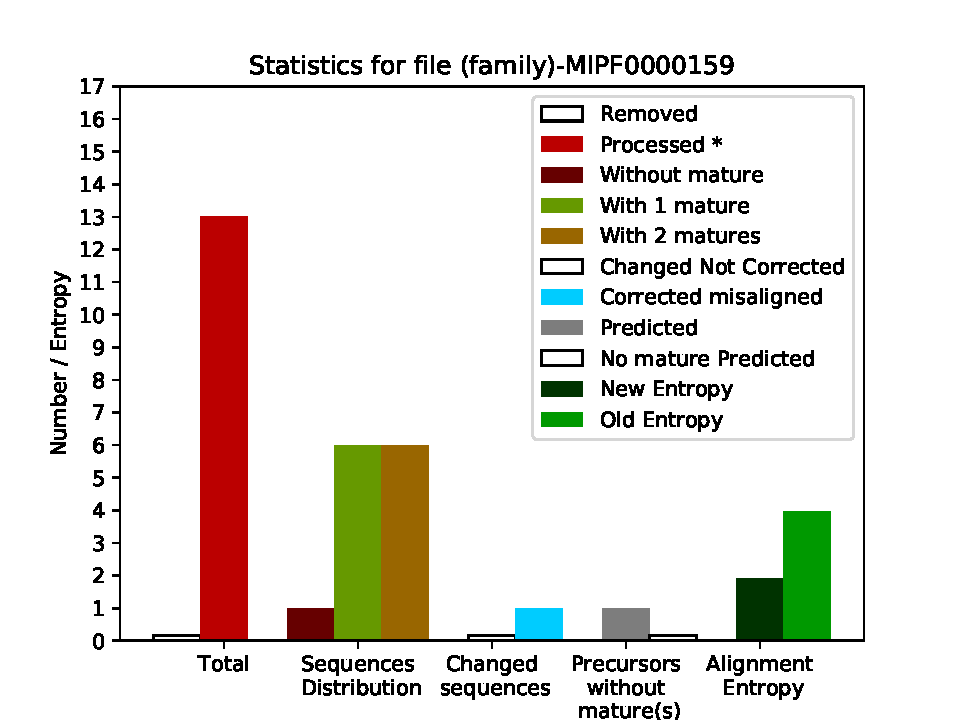
\includegraphics[width=\textwidth]{MIPF0000159statistics.pdf}
  \end{center}
  \caption{Example of the statistics output figure. The white columns are zeros.}
  \label{fig:MIPF0000159statistics.pdf}
\end{figure}

\subsubsection{Summary txt file}
\label{sec:sumtxt}
\noindent
This file includes  more statistical details and numbers, as well as the IDs of the precursors included in the statistics.\\ The name of 
this file: \textit{precursorsfilename-summ.txt}\\\\
(see \textit{examples\/main\_outputFiles/MIPF0000159-summ.txt} in the supplementary materials)

\subsubsection{JSON format file}
\noindent
Besides the txt summary file, a json file format contains the most useful statistical numbers to be easily 
parsed and read by machines.\\
The name of this file is: \textit{precursorsfilename.json}\\\\
(see \textit{examples\/main\_outputFiles/MIPF0000159.json} in the supplementary materials)


\end{document}
